\documentclass[a4paper, 12pt]{article}
\usepackage[T2A]{fontenc}
\usepackage[utf8]{inputenc}
\usepackage[russian, english]{babel}
\setlength{\parindent}{0pt}
\usepackage{amssymb,amsmath}
\usepackage{ifxetex,ifluatex}
\usepackage{fixltx2e} % provides \textsubscript
\ifnum 0\ifxetex 1\fi\ifluatex 1\fi=0 % if pdftex
  \usepackage[T2A]{fontenc}
  \usepackage[utf8]{inputenc}
\else % if luatex or xelatex
  \ifxetex
    \usepackage{mathspec}
  \else
    \usepackage{fontspec}
  \fi
  \defaultfontfeatures{Ligatures=TeX,Scale=MatchLowercase}
\fi
% use upquote if available, for straight quotes in verbatim environments
\IfFileExists{upquote.sty}{\usepackage{upquote}}{}
% use microtype if available
\IfFileExists{microtype.sty}{%
\usepackage{microtype}
\UseMicrotypeSet[protrusion]{basicmath} % disable protrusion for tt fonts
}{}
\usepackage[unicode=true]{hyperref}
\hypersetup{
            pdfborder={0 0 0},
            breaklinks=true}
\urlstyle{same}  % don't use monospace font for urls
\usepackage{graphicx,grffile}
\makeatletter
\def\maxwidth{\ifdim\Gin@nat@width>\linewidth\linewidth\else\Gin@nat@width\fi}
\def\maxheight{\ifdim\Gin@nat@height>\textheight\textheight\else\Gin@nat@height\fi}
\makeatother
% Scale images if necessary, so that they will not overflow the page
% margins by default, and it is still possible to overwrite the defaults
% using explicit options in \includegraphics[width, height, ...]{}
\setkeys{Gin}{width=\maxwidth,height=\maxheight,keepaspectratio}
\IfFileExists{parskip.sty}{%
\usepackage{parskip}
}{% else
\setlength{\parindent}{0pt}
\setlength{\parskip}{6pt plus 2pt minus 1pt}
}
\setlength{\emergencystretch}{3em}  % prevent overfull lines
\providecommand{\tightlist}{%
  \setlength{\itemsep}{0pt}\setlength{\parskip}{0pt}}
\setcounter{secnumdepth}{0}
% Redefines (sub)paragraphs to behave more like sections
\ifx\paragraph\undefined\else
\let\oldparagraph\paragraph
\renewcommand{\paragraph}[1]{\oldparagraph{#1}\mbox{}}
\fi
\ifx\subparagraph\undefined\else
\let\oldsubparagraph\subparagraph
\renewcommand{\subparagraph}[1]{\oldsubparagraph{#1}\mbox{}}
\fi
\usepackage{listings}

\date{}

\begin{document}

\tableofcontents

\pagebreak

\section{Генеративные модели}

\subsection{Лекция 1: Генеративные модели}

\begin{itemize}
\item
  
  Выход модели = Изображение
  

  \begin{itemize}
  \item
    
    Увеличение четкости
    
  \item
    
    Перенесение стиля
    
  \item
    
    \ldots{}
    
  \end{itemize}
\item
  
  \textbf{Евклидово расстояние}
  

  \begin{itemize}
  \item
    
    Сумма разниц между i-ми пикселями
    
  \item
    
    Не измеряет расстояние содержательно
    
  \end{itemize}
\item
  
  \textbf{Perceptual loss}
  

  \begin{itemize}
  \item
    
    Сравнивается контент изображений
    
  \item
    
    {Content loss}
    
  \end{itemize}
\end{itemize}

\[{L^{l}}_{\text{content}} = \sum_{ij} (A_{\text{ij}} - B_{\text{ij}})^{2}\]


\begin{itemize}
\item
  
  Берем i свертку на l слое и сравниваем отклики, j - отдельный элемент
  свертки
  
\end{itemize}

\begin{itemize}
\item
  
  Лучше брать последние слои
  
\item
  
  {Style loss}
  
\end{itemize}

\[{G^{l}}_{\text{ij}}(A)\  = \ {A^{l}}_{\text{ik}}{A^{l}}_{\text{jk}}\ \]

\begin{itemize}
\item
  
  Сравниваем похожесть каналов
  
\end{itemize}

\[{L^{l}}_{\text{style}}\  = \ ({G^{l}}_{\text{ij}}(A)\  - \ {G_{\text{ij}}}^{l}(B))^{2}\]

\[L_{\text{style}} = \sum_{l} {L^{l}}_{\text{style}}\]

\textbf{{Perceptual loss}}

\[L(C,\ S,\ X)\  = \ \alpha L_{\text{content}}(C,\ X)\  + \ \beta L_{\text{style}}(S,\ X)\  \rightarrow \text{mi}n_{X}\]

C - исходное изображение

S - стилевое изображение

X - выходное изображение

{Обучаемые параметры = пиксели выходной картинки}

{Недостатки}

\begin{itemize}
\item
  
  Очень долгая обработка
  
\end{itemize}

\textbf{Ускорение}

\begin{itemize}
\item
  
  Фиксируем стилевое изображение
  
\item
  
  Обучим модель \(\alpha(C)\), которая оптимизирует Perceptual loss
  
\item
  
  Теперь подбираем не пиксели, а обучаем модель
  
\item
  
  Оптимизируем по параметрам модели \(\alpha\)
  
\item
  
  ECCV16
  
\item
  
  Image Transform Network похожа на U-Net
  
\end{itemize}

\subsubsection{Superresolution}\label{superresolution}

\begin{itemize}
\item
  
  Повысить разрешение картинки
  
\item
  
  Подход в лоб
  

  \begin{itemize}
  \item
    
    Расширяем картинку
    
  \item
    
    Сетка выучивает дополнение к исходной картинке, чтобы MSE был
    минимальный между результатом и правильной картинкой
    
  \item
    
    The deeper, the better
    
  \end{itemize}
\item
  
  Можно использовать perceptual loss
  

  \begin{itemize}
  \item
    
    Но тогда появляются артефакты
    
  \end{itemize}
\end{itemize}

\subsubsection{Inpainting}\label{inpainting}

\begin{itemize}
\item
  
  Восстановить кусок картинки
  
\end{itemize}

\subsection{Лекция 2: Вариационные
автокодировщики}

\begin{itemize}
\item
  
  Denoising autoencoder
  
\end{itemize}
\begin{figure}[h]
    \centering
    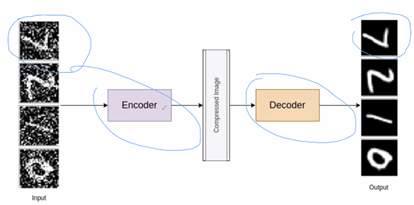
\includegraphics[width=4.31487in,height=2.13484in]{media/image4.png}
    \caption{Denoising}
    \label{fig:my_label}
\end{figure}

Если берем случайную точку, на которой модель не обучалась → Получаем
бред

{Вероятностные методы}

\begin{itemize}
\item
  
  Иногда проще описать в терминах вероятности
  
\item
  
  Подбираем параметры распределений так, чтобы обучающая выборка имела
  высокую вероятность
  
\item
  
  {Тематическое моделирование}
  

  \begin{itemize}
  \item
    
    {PLSA, LDA}
    
  \item
    
    Данные - набор текстов
    
  \item
    
    Каждая тема = распределение N слов
    
  \item
    
    Каждый текст = распределение на темах
    
  \item
    
    Генерация
    

    \begin{itemize}
    \item
      
      Выбираем тему
      
    \item
      
      Выбираем слова и добавляем в текст
      
    \end{itemize}
  \end{itemize}
\item
  
  {Изображения}
  

  \begin{itemize}
  \item
    
    Хотим построить пространство представлений
    
  \item
    
    Каждая картинка != точка, а \textbf{распределение}
    
  \item
    
    Возьмем нормальное распределение
    
  \end{itemize}
\end{itemize}


\[encoder(x)\  = \ (\mu(x),\ \sigma(x))\]


\begin{itemize}
\item
  
  МО и Дисперсия - вектор размера d
  
\item
  
  Сэмплируем вектор Z из распределения с\(\mu\)и \(\sigma\)
  
\item
  
  Декодировщик вектор разворачивает в картинку
  
\item
  
  Раскодированная картинка должна быть как можно ближе к исходной
  
\item
  
  Позволяет получить непрерывное пространство представлений
  
\item
  
  \(q(z|x)\)- кодировщик
  
\item
  
  \(p(x|z)\)- декодировщик \(decoder(z)\  + \ \epsilon\)
  
\item
  
  \((E_{q(z|x_{i})}log\ p(x_{i}|z)\  - \ KL(q(z|x)\ ||\ N(0,\ 1)))\  \rightarrow \max\)
  
\item
  
  KL - Дивергенция Кульбака - Лейблера
  

  \begin{itemize}
  \item
    
    Мера расстояния между распределениями
    
  \item
    
    \[KL(q,\ p)\  = \ q(x)log\frac{q(x)}{p(x)}\]
    
  \item
    
    Выполняет функцию регуляризации - чтобы не было узких распределений
    
  \end{itemize}
\item
  
  \textbf{Оптимизация - Reparametrization Trick}
  

  \begin{itemize}
  \item
    
    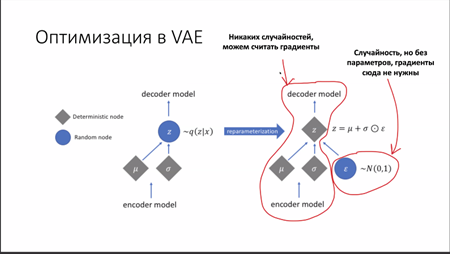
\includegraphics[width=4.68444in,height=2.64463in]{media/image17.png}
    
  \end{itemize}
\end{itemize}

\subsection{Лекция 3: GAN}
\begin{itemize}
\item
  
  Дано: выборка \(x_{i} = p_{x}(x)\), распределение неизвестно
  
\item
  
  Задача: генерировать новые объекты с таким же распределением
  
\item
  
  Генерируем z из двумерного нормального распределения → пространство Z
  называется {скрытым} → Пропускаем через генератор G(Z) → получаем
  \(\widehat{X} = G(Z)\)
  
\item
  
  Как посчитать сходство между \(X\ \text{и} \widehat{X}\)
  

  \begin{itemize}
  \item
    
    Строим задачу бинарной классификации \(X\ \text{и} \widehat{X}\) →
    {Дискриминатор}
    
  \item
    
    Используем значения log-loss для обучения дискриминатора
    
  \item
    
    \[L\  = \  - \ \frac{1}{n}y_{i}logD(x_{i})\  + \ (1\  - \ y_{i})log(1\  - \ D(x_{i}))\]
    
  \item
    
    \[L(D,\ G)\  = \  - \frac{1}{n}logD(x_{i})\  - \frac{1}{n}log(1\  - \ D(G(z_{i}))\]
    
  \item
    
    Обучение дискриминатора и генератора
    

    \begin{itemize}
    \item
      
      \[\text{ma}x_{G}\text{mi}n_{D}L(D,\ G)\]
      
    \end{itemize}
  \item
    
    \textbf{Проблемы GAN}
    

    \begin{itemize}
    \item
      
      Затухание градиентов
      
      \begin{itemize}
      \item
        
        Дискриминатор идеально разделяет выборки → Loss = 0
        
      \end{itemize}
    \item
      
      Схлопывание мод
      

      \begin{itemize}
      \item
        
        Несколько мод в распределении → получается выучить не все
        
      \item
        
        Для некоторых мод дискриминатор возвращает 1 → в окрестности нет
        градиентов
        
      \end{itemize}
    \end{itemize}
  \item
    
    \textbf{Wasserstein GAN}
    

    \begin{itemize}
    \item
      
      Меняем функцию потерь
      
    \item
      
      {Расстояние Вассерштейна}
      

      \begin{itemize}
      \item
        
        \(EMD(P_{r},\ P_{\theta})\  = \ inf\)..
        
      \item
        
        Дуальная форма: 
        
        \(EMD(P_{r},\ P_{\theta})\  = \ sup_{||f||L < 1}\)
      \end{itemize}
    \item Нет проблемы затухания градиентов
    \item Схлопывание мод
    \end{itemize}
  \item \textbf{Conditional GAN}
    \begin{itemize}
    \item Подаем дополнительно класс
    \end{itemize}
  \item \textbf{Cycle GAN}
    \begin{itemize}
    \item Есть дополнительная нейросеть, которая может переводить
      генерированные картинки обратно
    \end{itemize}
  \item \textbf{Bidirectional GAN}
  \end{itemize}
\end{itemize}

\subsection{Лекция 4: Нормализационные потоки}

\textbf{{Flow-based generative models}}

\begin{itemize}
\item
  
  Не 2 сети, а одна → Декодируем представление с помощью обратной
  функции
  
\item
  
  Не используем x' для обучения
  
\item
  
  VAE и GAN преобразуют скрытое пространство в данные
  {{необратимо}}
  
\item
  
  Нормализационные потоки выучивают {\textbf{обратимое}
  преобразование}
  
\item
  
  Позволяют рассчитать плотность вероятности для распределения
  

  \begin{itemize}
  \item
    
    Можно обнаружить аномалии / редкость
    
  \end{itemize}
\end{itemize}

\textbf{{Теорема о замене переменных}}

\begin{itemize}
\item
  
  Пространство признаков x
  
\item Скрытое пространство z
  \begin{itemize}
  \item Знаем функцию распределения
  \end{itemize}
\item \[(z\  = \ f(x)\]
  
\item Находим \(p_{x}\)
  
\item Знаем \(p_{z}(z),\ z\  = \ f(x)\)
  
\end{itemize}

\[p_{x}(x_{i})\  = \ p_{z}(f(x_{i}))|det\frac{\partial f(x_{i})}{\partial x_{i}}|\]

\[p_{z}(z_{i})\  = \ p_{x}(f^{- 1}(z_{i}))|det\frac{\partial f^{- 1}(z_{i})}{\partial z_{i}}|\]

\subsubsection{Нормализационные потоки}

\begin{itemize}
\item
  
  Есть признаки x - не знаем их распределение
  
\item
  
  Надо найти \(z\  = \ f(x)\), чтобы z имело известное распределение
  
\item
  
  Используем метод градиентного спуска
  

  \begin{itemize}
  \item
    
    Подбираем f с помощью {{логарифмической функции
    правдоподобия}}
  
  \end{itemize}
\end{itemize}

\[L\  = \  - \frac{1}{n}\text{log\ }p_{x}(x_{i})\]

\[p_{x}(x_{i})\  = \ p_{z}(f(x_{i}))|det\frac{\partial f(x_{i})}{\partial x_{i}}|\]

\[L\  = \  - \frac{1}{n}log\ (p_{z}(f(x_{i}))|det\frac{\partial f(x_{i})}{\partial x_{i}}|)\]

\[L\  = \  - \frac{1}{n}\text{log\ }p_{z}(f(x_{i})\  + \ log(|det\frac{\partial f(x_{i})}{\partial x_{i}}|)\  \rightarrow \min\]

\begin{itemize}
\item
  
  Прямая функция используется для переведения входных данных в случайный
  шум → Обратная функция генерирует картинки из полученного шума
  
\item
  
  {{Алгоритм обучения}}
  

  \begin{itemize}
  \item
    
    Берем минибатч
    
  \item
    
    Считаем лосс
    

    \begin{itemize}
    \item
      
      \(L\  = \  - \frac{1}{n}\text{log\ }p_{z}(f(x_{i})\  + \ log(|det\frac{\partial f(x_{i})}{\partial x_{i}}|)\)
      
    \end{itemize}
  \item Обновляем параметры функции f
  \end{itemize}
\item Алгоритм генерации
  \begin{itemize}
  \item Сэмплим точки из распределения z
  \item Генерируем объекты, используя обратную функцию \(f^{- 1}(z)\)
  \end{itemize}
\item
  
  Можно сделать {{несколько слоев}}
  

  \begin{itemize}
  \item
    
    Несколько промежуточных скрытых представлений
    
  \item
    
    За счет этого можно научиться генерировать более сложные объекты
    
  \item
    
    \(z_{i}\  = \ f_{2}(y_{i}),\ y_{i} = f_{1}(x_{i})\)
    
  \end{itemize}
\end{itemize}

\[p_{x}(x_{i})\  = \ p_{y}(f_{1}(x_{i}))|det\frac{\partial f_{1}(x_{i})}{\partial x_{i}}|\]

\[p_{y}(y_{i})\  = \ p_{z}(f_{2}(y_{i}))|det\frac{\partial f_{2}(y_{i})}{\partial y_{i}}|\]

\[p_{x}(x_{i})\  = p_{z}(f_{2}(y_{i}))|det\frac{\partial f_{2}(y_{i})}{\partial y_{i}}||det\frac{\partial f_{1}(x_{i})}{\partial x_{i}}|\]


\begin{itemize}
\item
  
  {{Выбор функции}}
  

  \begin{itemize}
  \item
    
    Дифференцируема?
    
  \item
    
    Обратима?
    
  \end{itemize}
\end{itemize}

\centering \textbf{Real-NVP}

\begin{itemize}
\item
  
  X и Z - d-мерные вектора
  
\end{itemize}


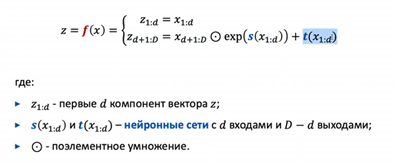
\includegraphics[width=4.12500in,height=1.73135in]{media/image6.png}

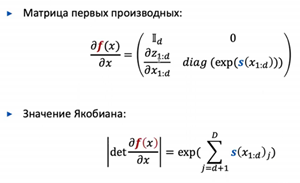
\includegraphics[width=3.12500in,height=1.90179in]{media/image19.png}

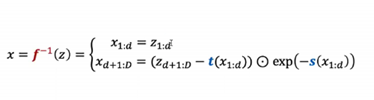
\includegraphics[width=3.89415in,height=1.04619in]{media/image23.png}

\textbf{{Masked Autoregressive Flow (MAF)}}


\centering 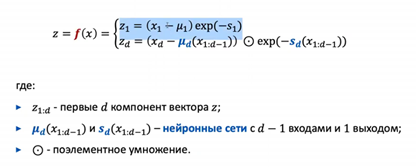
\includegraphics[width=4.33333in,height=1.73856in]{media/image8.png}

\centering 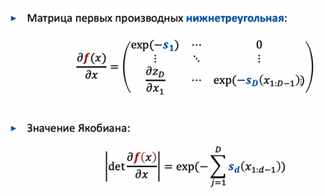
\includegraphics[width=3.38542in,height=2.04167in]{media/image24.png}

\centering 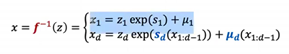
\includegraphics[width=3.01042in,height=0.56250in]{media/image15.png}

\begin{itemize}
\item
  
  Каждая компонента использует предыдущую → Дольше
  
\end{itemize}

\textbf{Inverse Autoregressive Flow (IAF)}


\centering 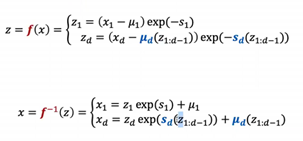
\includegraphics[width=3.15625in,height=1.46648in]{media/image11.png}


\begin{itemize}
\item
  
  Генерация быстрее, так как используем компоненты вектора z, который мы
  и так знаем
  
\item
  
  Обучение дольше, так как z обучается попиксельно
  
\end{itemize}

\section{Обработка звука}

\subsection{Лекция 5: Диалоговые системы}

\begin{itemize}
\item
  
  Прежде всего интересен текстовый формат
  

  \begin{itemize}
  \item
    
    Большинство данных в диалоговых системах переводится в текст
    
  \end{itemize}
\item
  
  Чат-боты
  

  \begin{itemize}
  \item
    
    Task-oriented → Узко специализированный
    
  \item
    
    Голосовые помощники = большое количество task-oriented скиллов
    
  \end{itemize}
\item
  
  {Типы ответов в диалоговых системах}
  

  \begin{itemize}
  \item
    
    Системы с готовыми ответами (Retrieval-based)
    

    \begin{itemize}
    \item
      
      Работает с пулом реплик
      
    \end{itemize}
  \item
    
    Generative-based
    
  \end{itemize}
\item Основные компатенты чат-бота
  \begin{itemize}
  \item Intent Detection
    \begin{itemize}
    \item Как обработать входную реплику, определить намерение пользователя
    \item Задача классификации → Какому приложению отправить реплику
    \item Выбор классификатора интента
      \begin{itemize}
      \item
        
        В облаке → Можно использовать сложную модель
        
      \item
        
        На устройстве → Поменьше
        
      \item
        
        Bert, Distilled Bert
        
      \item
        
        Можно даже не использовать машинное обучение → Ищем ключевые
        слова в предложениях
        
      \end{itemize}
    \end{itemize}
  \item
    
    Slot Filling
    

    \begin{itemize}
    \item
      
      Выделить из сообщения параметры
      
    \item
      
      ``Поставить будильник на {7 утра}''
      
    \item
      
      Слоты определяются на основе задачи
      

      \item Извлечение именованных сущностей
        

        \begin{itemize}
        \item Относится ли текущее слово к одному из классов, задающих слоты
        \item Рекуррентные нейронные сети → Извлекаем скрытое состояние
            для каждого отдельного слова
            
        \end{itemize}
      \item Можно делать последовательно → Сначала определяем интент →
        Выделяем слоты
        
      \item Можно решать задачи одновременно
    \end{itemize}
  \item
    
    {Граф сценария}
    

    \begin{itemize}
    \item
      
      Какие вещи нужно доспросить, какие слоты заполнить
      
    \end{itemize}
  \end{itemize}
\end{itemize}

\subsection{Вопросно-ответные системы, задача
SQuAD}

\begin{itemize}
\item
  
  Нейросетевая модель ищет ответ на вопрос
  
\item
  
  Должна:
  

  \begin{itemize}
  \item
    
    Понять вопрос на естественном языке
    
  \item
    
    Найти ответ в массиве данных
    
  \item
    
    Выдать ответ на естественном языке
    
  \end{itemize}
\item
  
  Типы вопросов
  

  \begin{itemize}
  \item
    
    Фактологические вопросы
    

    \begin{itemize}
    \item
      
      Легкие вопросы для нейронных сетей
      
    \end{itemize}
  \item
    
    Вопросы на понимание здравого смысла
    

    \begin{itemize}
    \item
      
      Сложны для нейросетей
      
    \end{itemize}
  \item
    
    Сравнительные вопросы
    

    \begin{itemize}
    \item
      
      Тоже сложно
      
    \end{itemize}
  \end{itemize}
\item
  
  Подходы к построению QA систем
  

  \begin{itemize}
  \item
    
    {Информационный поиск}
    

    \begin{itemize}
    \item
      
      Текстовая коллекция, разбитая на фрагменты
      
    \end{itemize}
  \item
    
    {Поиск по базе знаний}
    

    \begin{itemize}
    \item
      
      Формируем запрос к базе знаний как функцию → Она выдает ответ
      
    \item
      
      Более сложный подход
      
    \end{itemize}
  \end{itemize}
\item
  
  {Задача SQuAD}
  

  \begin{itemize}
  \item
    
    Ищем ответ на вопрос в тексте
    
  \item
    
    Stanford Question Answering Dataset
    

    \begin{itemize}
    \item
      
      Текст вопроса
      
    \item
      
      Текстовый фрагмент, содержащий ответ
      
    \item
      
      Текст ответа
      
    \end{itemize}
  \item
    
    \textbf{Решение задачи SQuAD}
    

    \begin{itemize}
    \item
      
      Отбор параграфов, которые могут содержать ответ на вопрос
      

      \begin{itemize}
      \item
        
        Обычно используют грубые и быстрые методы
        

      \item
        
        Косинусное расстояние между TF-IDF / FastText вопроса и
        параграфа
          
      \end{itemize}
    \item
      
      Поиск подстрок фрагмента с ответом
      

      \begin{itemize}
      \item
        
        Трансформеры
        
      \item
        
        Ищем максимальное произведение вероятностей, что первый токен
        последовательности - начало ответа, а последний токен - конец
        ответа
        
      \end{itemize}
    \end{itemize}
  \end{itemize}
\end{itemize}

\subsection{Лекция 6: Обработка звука}

\begin{itemize}
\item
  
  Звук - колебания воздуха
  
\item
  
  Аналоговый сигнал подвергается дискретизации, квантованию, кодированию
  

  \begin{itemize}
  \item
    
    {Квантование}
    

    \begin{itemize}
    \item
      
      Сигнал разбивается на N уровней
      
    \item
      
      Для каждой точки берется ближайший уровень
      
    \end{itemize}
  \item
    
    {Дискретизация}
    

    \begin{itemize}
    \item
      
      Сигнал представляется в виде последовательных значений, взятых в
      дискретные моменты времени t с шагом d
      
    \item
      
      В виде точек, а не функции
      
    \end{itemize}
  \end{itemize}
\end{itemize}

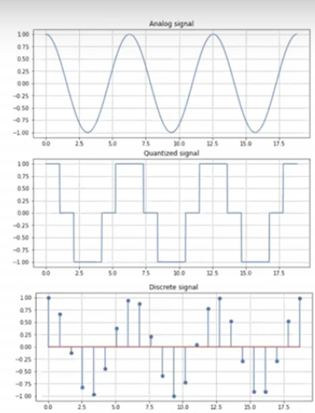
\includegraphics[width=3.28286in,height=4.29876in]{media/image25.png}

\begin{itemize}
\item
  
  {Характеристики}
  

  \begin{itemize}
  \item
    
    Частота дискретизации - количество отсчетов амплитуды в секунду
    
  \item
    
    Количество каналов
    
  \end{itemize}
\item Почему плохо работать со звуком в таком формате
  

  \begin{itemize}
  \item
    
    Один звук состоит из 2000-4000 амплитуд → дорого хранить и
    обрабатывать
    
  \item
    
    Нет инварианта относительно шума и трансформаций → лучше
    использовать спектрограмму
    
  \end{itemize}
\item
  
  {Дискретное преобразование Фурье}
  
\end{itemize}


\(X\  = \ Mx\)

\(Mmn\  = \ exp( - 2\pi i\frac{(m\  - \ 1)(n\  - \ 1)}{N})\)


\begin{itemize}
\item
  
  {Спектрограмма}
  

  \begin{itemize}
  \item
    
    Нарезаем сигнал на окна с пересечением
    
  \item
    
    Применяем оконную функцию к вырезанному окну
    
  \item
    
    Применяем дискретное преобразование Фурье
    
  \item
    
    Считаем квадрат комплексной нормы
    
  \item
    
    Берем половину вектора + 1 в силу его симметричности
    

    \begin{itemize}
    \item
      
      Свойство преобразования Фурье
      
    \end{itemize}
  \end{itemize}
\item
  
  {Мелспектрограмма}
  
\end{itemize}


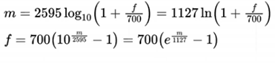
\includegraphics[width=2.86827in,height=0.65760in]{media/image22.png}


\begin{itemize}
\item
  
  В конце берем \textbf{логарифм} от спектрограммы
  
\item
  
  Из нее хуже звук восстанавливается
  
\item
  
  Обратимость операции не точная
  
\end{itemize}

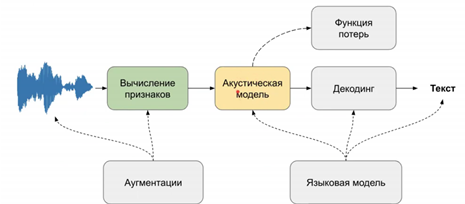
\includegraphics[width=4.84375in,height=2.12500in]{media/image5.png}

\begin{itemize}
\item
  
  {Метрики}
  
\end{itemize}

\(Word\ Error\ Rate\  = \ \frac{S\  + \ D\  + \ I}{S\  + \ D\  + \ C}\)

\begin{itemize}
\item
  
  S - кол-во замен
  
\item
  
  D - кол-во удалений
  
\item
  
  I - кол-во вставок
  
\item
  
  C - кол-во совпадений
  
\item
  
  \textbf{CER} - посимвольное совпадение
  
\end{itemize}

\begin{itemize}
\item \subsection{Listen, Attend, Spell}
  \begin{itemize}
  \item
    
    Listener = пирамидальный LSTM-encoder
    
  \end{itemize}
\end{itemize}


Выходы для каждого слоя конкатенируем и подаем в следующую лстм


\begin{itemize}
\item
  
  Speller = LSTM декодер
  
\item
  
  Attention
  
\item
  
  Минимизируем кросс-энтропию с правильными буквами
  
\item
  
  Учим с помощью teach-forcing'а
  
\item
  
  Декодируем с помощью beam search
  
\item
  
  Добавляем языковую модель для улучшения результата
  
\item
  
  {Second pass fusing}
  
\end{itemize}

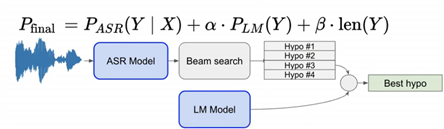
\includegraphics[width=4.62500in,height=1.34375in]{media/image9.png}

\begin{itemize}
\item
  
  {Shallow fusing}
  

  \begin{itemize}
  \item
    
    Добавляем языковую модель в beam search
    
  \end{itemize}
\end{itemize}

\subsection{\texorpdfstring{\textbf{Лекция 7: Обработка звука
2}}{Лекция 7: Обработка звука 2}}\label{ux43bux435ux43aux446ux438ux44f-7-ux43eux431ux440ux430ux431ux43eux442ux43aux430-ux437ux432ux443ux43aux430-2}

\subsection{Connectionist Temporal
Classification}\label{connectionist-temporal-classification}

\begin{itemize}
\item
  
  Вход и выход разной длины и они не выровнены
  
\item
  
  {Алгоритм}
  

  \begin{itemize}
  \item
    
    Для каждого фрейма делаем предсказание буквы
    
  \item
    
    Склеиваем соседние одинаковые предсказания
    
  \item
    
    Для поиска пробелов используют эпсилон-токены
    

    \begin{itemize}
    \item
      
      Тишина
      
    \end{itemize}
  \item
    
    Удаляем эпсилон-токены и склеиваем предложение
    
  \end{itemize}
\item
  
  {Как считать и пробрасывать градиенты}
  

  \begin{itemize}
  \item
    
    Импортировать из торча
    
  \item
    
    Динамическое программирование
    
  \end{itemize}
\end{itemize}

\subsection{Jasper}\label{jasper}

\begin{itemize}
\item
  
  Сверточная модель
  
\item
  
  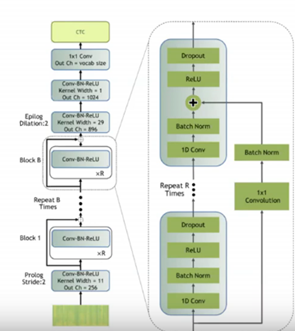
\includegraphics[width=3.07813in,height=3.44708in]{media/image12.png}
  
\item
  
  Из-за skip-connections быстро сходится
  
\item
  
  Функция потерь CTC
  
\item
  
  1-D convolutions
  

  \begin{itemize}
  \item
    
    Одномерный сигнал с большим количеством каналов
    
  \item
    
    Канал = частота
    
  \item
    
    Размерность 1 = время
    
  \end{itemize}
\end{itemize}

\subsection{Аугментации}\label{ux430ux443ux433ux43cux435ux43dux442ux430ux446ux438ux438}

\begin{itemize}
\item
  
  Данных не очень много
  
\item
  
  Помогают с нехваткой данных и улучшают робастность
  
\item
  
  Либо по времени, либо по частотам вырезаем кусок спектрограммы,
  заменяя нулевыми амплитудами
  
\end{itemize}

\subsection{Синтезация
голоса}\label{ux441ux438ux43dux442ux435ux437ux430ux446ux438ux44f-ux433ux43eux43bux43eux441ux430}

\subsubsection{Пайплайн
TTS}\label{ux43fux430ux439ux43fux43bux430ux439ux43d-tts}

\begin{itemize}
\item
  
  Hello
  
\item
  
  Text Frontend
  

  \begin{itemize}
  \item
    
    Нормализация текста
    

    \begin{itemize}
    \item
      
      Убираем специальные символы
      
    \end{itemize}
  \item
    
    Транскрибируем фонемы
    

    \begin{itemize}
    \item
      
      Переводит буквы в звукы (написание не совпадает с произношением)
      
    \end{itemize}
  \end{itemize}
\item Mel Synthesis
  

  \begin{itemize}
  \item
    
    Синтезируем частоты
    
  \end{itemize}
\item
  
  WAV Synthesis
  
\end{itemize}

\subsubsection{Как измерять
качество}\label{ux43aux430ux43a-ux438ux437ux43cux435ux440ux44fux442ux44c-ux43aux430ux447ux435ux441ux442ux432ux43e}

\begin{itemize}
\item
  
  Сложно оценить качество
  
\item
  
  Нет правильного ответа
  
\item
  
  Субъективность правильности
  
\item
  
  Синтез оценивается с помощью краудсорса
  
\end{itemize}

\subsubsection{Wave-Net}\label{wave-net}

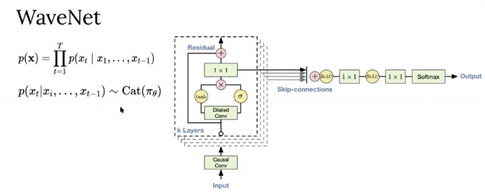
\includegraphics[width=5.05085in,height=2.00567in]{media/image2.png}

\begin{itemize}
\item
  
  {Causal Conv}
  

  \begin{itemize}
  \item
    
    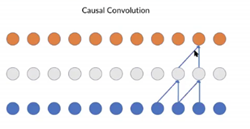
\includegraphics[width=2.60938in,height=1.34624in]{media/image10.png}
    
  \item
    
    Не используем паддинг
    
  \end{itemize}
\item
  
  {Mu law encoding}
  

  \begin{itemize}
  \item
    
    \(f(x_{t})\  = \ sign(x_{t})\frac{ln(1\  + \ \mu|x_{t}|)}{ln(1\  + \ \mu)}\)
    
  \item
    
    В высоком разрешении храним низкие амплитуды, в низком высокие
    
  \item
    
    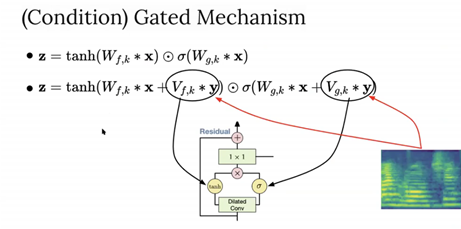
\includegraphics[width=4.80208in,height=2.38648in]{media/image7.png}
    
  \item
    
    \(W_{f,k},\ W_{j,k\ }\)- некоторые свертки
    
  \item
    
    Gated Mechanism - выучивает на какие куски аудио смотреть (как LSTM)
    
  \item
    
    \(V_{f,\ k}*y,\ V_{g,\ k}*y\)- генерируем с помощью сверток, y - уже
    сгенерированная Мел-спектрограмма
    
  \item
    
    x - Все предыдущие предсказанные сэмплы
    
  \end{itemize}
\item
  
  {Функция потерь}
  

  \begin{itemize}
  \item
    
    Категориальное распределение
    
  \item
    
    Нормальное распределение
    
  \item
    
    Логистическое распределение
    
  \end{itemize}
\item
  
  Модель выдает распределение
  
\item
  
  Skip-connections идут к выводу
  
\end{itemize}

\subsubsection{Mel-GAN}\label{mel-gan}

\begin{itemize}
\item
  
  Получаем Mel из предыдущей системы
  
\item
  
  Генератор:
  
\item
  
  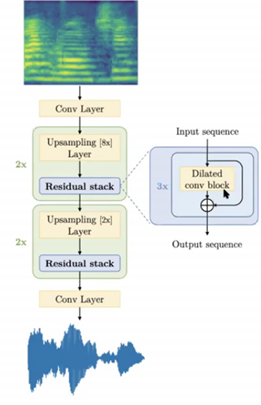
\includegraphics[width=2.72396in,height=4.21565in]{media/image21.png}
  
\item
  
  Дискриминатор:
  
\item
  
  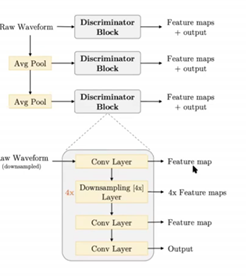
\includegraphics[width=2.56771in,height=2.87530in]{media/image20.png}
  
\item
  
  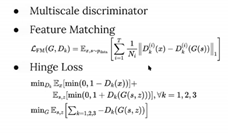
\includegraphics[width=2.38021in,height=1.41285in]{media/image1.png}
  
\end{itemize}

\section{\texorpdfstring{\textbf{Рекомендательные
системы}}{Рекомендательные системы}}\label{ux440ux435ux43aux43eux43cux435ux43dux434ux430ux442ux435ux43bux44cux43dux44bux435-ux441ux438ux441ux442ux435ux43cux44b}

\subsection{\texorpdfstring{\textbf{Лекция 8: Рекомендательные
системы}}{Лекция 8: Рекомендательные системы}}\label{ux43bux435ux43aux446ux438ux44f-8-ux440ux435ux43aux43eux43cux435ux43dux434ux430ux442ux435ux43bux44cux43dux44bux435-ux441ux438ux441ux442ux435ux43cux44b}

\ldots{}

\textbf{User-based рекомендации}

Оцениваем сходство с другими пользователями → Рекомендуем пользователю
то, что нравится похожим на него, но он не видел

{Проблемы Memory-based}

\begin{itemize}
\item
  
  Долго
  
\item
  
  Нет обучения, алгоритм не подкручивается
  
\item
  
  Проблема холодного старта → Новые объекты и пользователи = проблема
  
\end{itemize}

\textbf{Item-based рекомендации}

\begin{itemize}
\item
  
  Считаем сходства по тому, как объекты понравились разным пользователям
  → находим ближайшие
  
\end{itemize}

\textbf{Модели со скрытыми переменными}

{(Latent factor model)}

Строим векторы p, q → \textless{}p, q\textgreater{} \(\approx\) рейтинг

d - число жанров видео

\(p_{u}\)- как каждому пользователю нравятся жанры

\(q\)- распределение жанров в видео

\textless{}p, q\textgreater{} отражает совпадение интересов

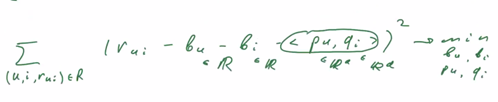
\includegraphics[width=5.18611in,height=1.06005in]{media/image3.png}

\begin{itemize}
\item
  
  \(b_{u},\ b_{i}\) - сдвиги
  
\end{itemize}

\begin{itemize}
\item
  
  Можно добавлять рекомендацию
  
\item
  
  \(P\  = \ (p_{1}|\ p_{2}|\ ...\ |p_{n})\)
  
\item
  
  \(Q\  = (q_{1}|q_{2}|\ ...\ |q_{m})\ \)
  
\item
  
  \((P^{T}Q)_{\text{ui}} = \  < p_{u},\ q_{i} >\)
  
\item
  
  Приближение матрицы матрицей меньшего ранга
  
\end{itemize}

{Как обучать?}

\begin{itemize}
\item
  
  Просто стохастическим спуском → выбираем u, i → работает не очень
  
\item
  
  ALS (alternating least squares)
  

  \begin{itemize}
  \item
    
    a)
    

    \begin{itemize}
    \item
      
      Матрицы P, Q инициализируем
      
    \item
      
      Фиксируем матрицу
      Q
      
      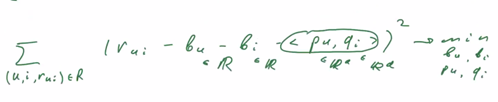
\includegraphics[width=5.18611in,height=1.06005in]{media/image3.png}
      
    \item
      
      \(q_{i}\) теперь фиксированное, а p нужно найти
      
    \item
      
      Получается задача обучения линейной модели
      
    \end{itemize}
  \item
    
    b)
    

    \begin{itemize}
    \item
      
      Фиксируем матрицу P
      
    \item
      
      \ldots{}
      
    \end{itemize}
  \item
    
    Практический нюанс:
    

    \begin{itemize}
    \item
      
      Делаем ALS
      
    \item
      
      Храним только Q
      
    \item
      
      Приходит новый пользователь
      
    \item
      
      Делаем один шаг ALS при фиксированной матрице Q
      
    \item
      
      Делаем \textless{}p, q\textgreater{}
      
    \end{itemize}
  \item
    
    Модификация для учета неявной информации
    

    \begin{itemize}
    \item
      
      Ситуация, когда рейтинги очень специфичные
      
    \item
      
      Для (u, i) мы либо знаем, что взаимодействие было, либо не знаем
      ничего
      

      \begin{itemize}
      \item
        
        Не знаем понравилось ли пользователю
        
      \end{itemize}
    \item
      
      {IALS}
      

      \begin{itemize}
      \item
        
        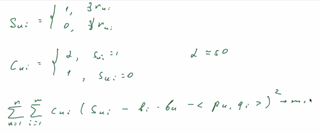
\includegraphics[width=3.33333in,height=1.38430in]{media/image16.png}
        
      \item
        
        Все объекты, с которыми пользователь взаимодействовал =
        положительный пример
        
      \item
        
        Пользователь не взаимодействовал → Ставим маленький вес при
        помощи Cui
        
      \end{itemize}
    \end{itemize}
  \end{itemize}
\end{itemize}

\subsection{\texorpdfstring{\textbf{Лекция 9: Рекомендательные системы
2}}{Лекция 9: Рекомендательные системы 2}}\label{ux43bux435ux43aux446ux438ux44f-9-ux440ux435ux43aux43eux43cux435ux43dux434ux430ux442ux435ux43bux44cux43dux44bux435-ux441ux438ux441ux442ux435ux43cux44b-2}

\textbf{Метрики качества рекомендаций}

\begin{enumerate}
\def\labelenumi{\arabic{enumi}.}
\item
  
  Насколько рекомендации подходят
  

  \begin{enumerate}
  \def\labelenumii{\alph{enumii}.}
  \item
    
    На чем измерять качество
    

    \begin{enumerate}
    \def\labelenumiii{\roman{enumiii}.}
    \item
      
      Оффлайн - измеряем на исторических данных
      

      \begin{enumerate}
      \def\labelenumiv{\arabic{enumiv}.}
      \item
        
        Режем по событиям юзера
        
      \item
        
        Режем по времени
        
      \end{enumerate}
    \item
      
      Онлайн - A/B тестирование
      

      \begin{enumerate}
      \def\labelenumiv{\arabic{enumiv}.}
      \item
        
        Берем две группы пользователей, рандомно, чтобы они не
        отличались
        
      \item
        
        В одной группе делаем рекомендации старым методом, а в другой
        новым методом
        
      \item
        
        Сравниваем метрики
        
      \end{enumerate}
    \end{enumerate}
  \item
    
    Регрессия
    

    \begin{enumerate}
    \def\labelenumiii{\roman{enumiii}.}
    \item
      
      MSE, MAE, \ldots{}
      
    \end{enumerate}
  \item
    
    Классификация
    

    \begin{enumerate}
    \def\labelenumiii{\roman{enumiii}.}
    \item
      
      F-мера, AUC-ROC, \ldots{}
      
    \end{enumerate}
  \item
    
    Качество ранжирования
    

    \begin{enumerate}
    \def\labelenumiii{\roman{enumiii}.}
    \item
      
      Система выдает ранжированный список
      
    \item
      
      Показываем пользователю top-k айтемов
      
    \item
      
      \(R_{u}(K)\) - top-k рекомендаций
      
    \item
      
      \(L_{u}\)- айтемы, которые пользователю понравились
      
    \item
      
      hitrate@k =
      {[}\(R_{u}(K)\  \cap \ L_{u}\  \neq pustomu\ mnozhestvu\rbrack\)
      
    \item
      
      precision@k = \({|R}_{u}(K)\  \cap \ L_{u}|\ /\ K\)- не учитывает
      ранжирование
      
    \item
      
      recall@k = \({|R}_{u}(K)\  \cap \ L_{u}|\ /\ |L_{u}|\)
      
    \item
      
      DCG
      

      \begin{enumerate}
      \def\labelenumiv{\arabic{enumiv}.}
      \item
        
        \(a_{\text{ui}} = a(u,\ i)\)
        
      \item
        
        Сортируем айтемы по невозрастанию \(a_{\text{ui}}\)
        
      \item
        
        \(r_{ui1},\ ...,\ r_{\text{uip}}\)- истинные рейтинги
        
      \item
        
        DCG@k = \(g(r_{\text{uip}}) \times d(p)\)
        
      \item
        
        d - штраф за позицию
        
      \item
        
        g(r) = \(2^{r} - 1\) или g(r) = r
        
      \item
        
        d(p) = \(\frac{1}{log(p\  + \ 1)}\)
        
      \end{enumerate}
    \item
      
      nDCG@k - нормализованный
      

      \begin{enumerate}
      \def\labelenumiv{\arabic{enumiv}.}
      \item
        
        DCG(u) / maxDCG(u)
        
      \end{enumerate}
    \end{enumerate}
  \end{enumerate}
\item
  
  Другие метрики
  

  \begin{enumerate}
  \def\labelenumii{\alph{enumii}.}
  \item
    
    Новизна (novelty)
    

    \begin{enumerate}
    \def\labelenumiii{\roman{enumiii}.}
    \item
      
      Число айтемов, которые раньше не рекомендовались
      
    \item
      
      Опросы (никто не отвечает)
      
    \end{enumerate}
  \item
    
    Разнообразие (diversity)
    

    \begin{enumerate}
    \def\labelenumiii{\roman{enumiii}.}
    \item
      
      Измеряем попарное расстояние между эмбеддингами айтемов
      
    \item
      
      Смотреть на дисперсию метаданных
      
    \item
      
      Предсказания модели для каждого айтема независимы, но в реальности
      это не так → Разнообразие повышает пользовательские метрики
      
    \end{enumerate}
  \item
    
    Serendipity - умение рекомендовать очень редкие айтемы, которые
    понравятся пользователю
    

    \begin{enumerate}
    \def\labelenumiii{\roman{enumiii}.}
    \item
      
      b - новая
      
    \item
      
      B - мн-во книг, которые пользователь оценил
      
    \item
      
      \(C_{\text{Bw}}\)- число книг автора w в множестве B
      
    \item
      
      \(S_{B}\)- максимальное число книг одного автора в B
      
    \item
      
      \(d(b,\ B)\  = \ \frac{1\  + \ C_{B} - C_{B,w\ }}{1\  + \ C_{B}}\)
      
    \end{enumerate}
  \item
    
    Что с этим всем делать?
    

    \begin{enumerate}
    \def\labelenumiii{\roman{enumiii}.}
    \item
      
      Подход 1
      

      \begin{enumerate}
      \def\labelenumiv{\arabic{enumiv}.}
      \item
        
        Есть бизнес-метрика M, есть остальные метрики f, \ldots{}, f
        
      \item
        
        Ищем веса при метриках, чтобы они приближали M
        
      \end{enumerate}
    \item
      
      Подход 2 (Ухудшающие эксперименты)
      

      \begin{enumerate}
      \def\labelenumiv{\arabic{enumiv}.}
      \item
        
        Рандом, предлагать только популярное, \ldots{}
        
      \item
        
        Подбираем веса так, чтобы во всех ухудшающих экспериментах
        взвешенная сумма уменьшалась
        
      \end{enumerate}
    \end{enumerate}
  \end{enumerate}
\end{enumerate}

\textbf{О разном}

\begin{itemize}
\item
  
  Как делать отбор кандидатов
  

  \begin{itemize}
  \item
    
    Сократить всю базу до более маленькой выборки
    
  \item
    
    Простые методы
    

    \begin{itemize}
    \item
      
      Те же жанры, исполнители, \ldots{}
      
    \item
      
      Самое популярное сейчас
      
    \end{itemize}
  \item
    
    На основе матричных разложений
    

    \begin{itemize}
    \item
      
      Пользователь-исполнитель
      
    \end{itemize}
  \item
    
    На основе сходства
    

    \begin{itemize}
    \item
      
      Уже есть эмбеддинги для пользователей и айтемов
      
    \end{itemize}
  \end{itemize}
\item
  
  Холодный старт
  

  \begin{itemize}
  \item
    
    Новый пользователь
    

    \begin{itemize}
    \item
      
      Самое популярное?
      
    \item
      
      Опрос об интересах
      
    \end{itemize}
  \item
    
    Новый айтем
    

    \begin{itemize}
    \item
      
      Показать фанатам этого же исполнителя
      
    \item
      
      Exploration - случайным пользователям показывать
      
    \end{itemize}
  \end{itemize}
\item
  
  Контентные рекомендации
  

  \begin{itemize}
  \item
    
    Можно делать факторы из эмбеддингов
    
  \item
    
    Факторы:
    

    \begin{itemize}
    \item
      
      Расстояние между контентным эмбеддингом этого айтемы и айтемов,
      которые нравились до этого
      
    \item
      
      DSSM
      

      \begin{itemize}
      \item
        
        Deep semantic similarity model
        
      \item
        
        Сеть с двумя половинами (user / item)
        
      \item
        
        Item
        

      \item
        
        Строим эмбеддинг по контенту
          
      \item
        
        User
        

      \item Строим эмбеддинг по контенту всех айтемов, которые раньше
          понравились пользователю
          
      \item
        
        Выучиваем эмбеддинги так, чтобы эмбеддинги были близки для
        близких объектов → Триплетный лосс
        
      \end{itemize}
    \end{itemize}
  \end{itemize}
\item
  
  Нейросетевая коллаборативная фильтрация (NCF)
  

  \begin{itemize}
  \item
    
    Есть эмбеддинг пользователя, есть айтема
    
  \item
    
    Конкатенируем
    
  \item
    
    Сверху полносвязные слои
    
  \item
    
    Результаты лучше, чем обычное матричное разложение (LFM)
    
  \item
    
    Steffen Rendle - критиковал эту технологию → Нейросети очень сложно
    аппроксимировать просто скалярное произведение
    
  \end{itemize}
\end{itemize}

\section{\texorpdfstring{\textbf{Продуктовая
аналитика}}{Продуктовая аналитика}}\label{ux43fux440ux43eux434ux443ux43aux442ux43eux432ux430ux44f-ux430ux43dux430ux43bux438ux442ux438ux43aux430}

\subsection{\texorpdfstring{\textbf{Лекция 10:
A/B-тестирование}}{Лекция 10: A/B-тестирование}}\label{ux43bux435ux43aux446ux438ux44f-10-ab-ux442ux435ux441ux442ux438ux440ux43eux432ux430ux43dux438ux435}

\textbf{Двойное слепое рандомизированное плацебо-контролируемое
исследование}

\begin{itemize}
\item
  
  Разделение на две {случайные} группы
  
\item
  
  Пациент не знает и врач не знает
  
\end{itemize}

\textbf{Тройное слепое \ldots{}}

\begin{itemize}
\item
  
  Исследователи должны тоже не знать
  
\end{itemize}

\textbf{Для чего нужно?}

\begin{itemize}
\item
  
  Оценка полезности нового явления
  
\item
  
  Исследование зависимостей
  

  \begin{itemize}
  \item
    
    Ухудшающие эксперименты → подбор новых метрик
    
  \end{itemize}
\item
  
  Мониторинги
  

  \begin{itemize}
  \item
    
    Вечный обратный эксперимент - возвращаем части пользователей то как
    было раньше
    
  \end{itemize}
\item
  
  Построение целей и KPI
  
\end{itemize}

\textbf{Из чего состоит эксперимент}

\begin{itemize}
\item
  
  Разбиение пользователей
  

  \begin{itemize}
  \item
    
    Может быть сложно получить случайные группы, в программировании
    рандомизация работает неплохо
    
  \item
    
    Как разбивать новых пользователей?
    
  \item
    
    Несколько экспериментов одновременно? → по 5\% можно проводить 20
    экспериментов за раз → Усложняет задачу разбиения
    
  \item
    
    Как можно детектировать качество разбиения?
    
  \item
    
    {Виды}
    

    \begin{itemize}
    \item
      
      По пользователям - cookies
      
    \item
      
      По визитам
      
    \item
      
      По действиям
      
    \end{itemize}
  \end{itemize}
\item
  
  Конфигурация эксперимента
  

  \begin{itemize}
  \item
    
    Длительность - trade-off
    
  \item
    
    Размер выборок
    
  \item
    
    Срез
    
  \end{itemize}
\item
  
  Метрики
  
\item
  
  Интерпретация результата
  
\item
  
  Корректность эксперимента
  
\end{itemize}

\textbf{Виды экспериментов}

\begin{itemize}
\item
  
  Одномерный / Многомерный
  
\end{itemize}

\begin{itemize}
\item
  
  Прямой / Обратный
  
\item
  
  Временный / Вечный
  
\item
  
  АА / AB
  
\end{itemize}

{Конфигурация}

\begin{itemize}
\item
  
  Размер выборок
  

  \begin{itemize}
  \item
    
    Trade-off - при больших выборках можно продержать пользователей на
    плохом продукте + невозможность тестировать большое количество
    экспериментов vs Состоятельность эксперимента
    
  \item
    
    При большой выборке можно использовать нормальные распределения +
    доверительный интервал меньше
    
  \item
    
    Чтобы доверительный интервал сократился в 2 раза надо в 4 раза
    увеличить размер выборки
    
  \end{itemize}
\item
  
  Длительность
  

  \begin{itemize}
  \item
    
    Нужно учитывать сезонность
    
  \end{itemize}
\item
  
  Срез
  
\end{itemize}

{Метрика}

\begin{itemize}
\item
  
  Чувствительность
  
\item
  
  Шум
  

  \begin{itemize}
  \item
    
    Большая дисперсия на среднее
    
  \item
    
    Работает только на большом количестве пользователей
    
  \end{itemize}
\item
  
  Интерпретация
  
\item
  
  Иерархия
  

  \begin{itemize}
  \item
    
    Связь с бизнес показателями
    
  \item
    
    Интерпретируемость
    
  \item
    
    Можно найти прокси-метрики для больших метрик и доказать влияние
    
  \end{itemize}
\end{itemize}

{Статистические тесты}

\begin{itemize}
\item
  
  T-test
  
\item
  
  Mann-Whitney
  
\end{itemize}

\subsection{\texorpdfstring{\textbf{Лекция 11: А/B тестирование
(2)}}{Лекция 11: А/B тестирование (2)}}\label{ux43bux435ux43aux446ux438ux44f-11-ux430b-ux442ux435ux441ux442ux438ux440ux43eux432ux430ux43dux438ux435-2}

\begin{itemize}
\item
  
  Статистический критерий - правило, которое позволяет делать вывод о
  том, стоит отвергать гипотезу или нет
  
\item
  
  P-value - вероятность ошибки, при условии, что нулевая гипотеза верна
  
\item
  
  Доверительный интервал → Если один лежит правее или левее другого,
  можно сделать вывод о значимости изменения
  
\item
  
  \textbf{Z-тест / T-тест}
  

  \begin{itemize}
  \item
    
    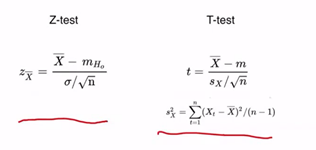
\includegraphics[width=3.29167in,height=1.56443in]{media/image18.png}
    
  \item
    
    Для гипотезы о средних
    
  \item
    
    Можем понять доверительные интервалы из этих тестов
    
  \item
    
    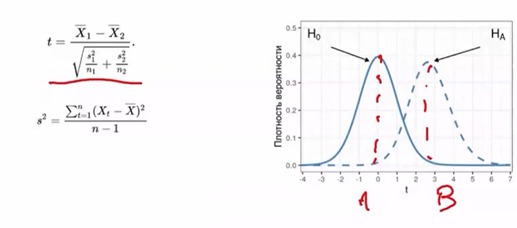
\includegraphics[width=5.38962in,height=2.37382in]{media/image13.png}
    
  \item
    
    Нужно знать, что распределение среднего близко к нормальному
    
  \end{itemize}
\item
  
  \textbf{Критерий Mann-Whitney}
  

  \begin{itemize}
  \item
    
    Берем массив и сортируем
    
  \item
    
    Смотрим какой выборке принадлежит каждое значение
    
  \item
    
    Ранговый критерий
    

    \begin{itemize}
    \item
      
      Выписываем ранги X и Y
      
    \item
      
      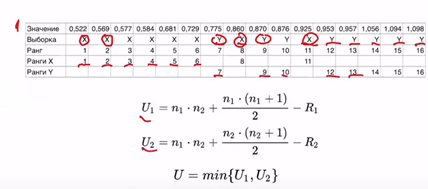
\includegraphics[width=4.45833in,height=1.97270in]{media/image14.png}
      
    \item
      
      {Робастный способ + не зависит от распределения}
      
    \end{itemize}
  \end{itemize}
\end{itemize}

\textbf{{Примеры}}

\begin{itemize}
\item
  
  Эксперимент 1
  

  \begin{itemize}
  \item
    
    Ухудшение метрики через время (пользователи привыкли?)
    

    \begin{itemize}
    \item
      
      Может быть просто сезонность - продлить эксперимент
      
    \item
      
      Взять срез для пользователей, которые пользовались с первого дня и
      посмотреть метрику для них
      
    \item
      
      Подождать 21 день и сделать обратный эксперимент
      
    \item
      
      Убедится, что эксперимент работает корректно
      
    \end{itemize}
  \end{itemize}
\item
  
  Эксперимент 2
  

  \begin{itemize}
  \item
    
    По первым 4м дням видим улучшение метрик
    

    \begin{itemize}
    \item
      
      Сезонность
      
    \item
      
      Проверяем метрику каждый час = фактически множественная проверка
      гипотез
      
    \end{itemize}
  \end{itemize}
\item
  
  Эксперимент 3
  

  \begin{itemize}
  \item
    
    По первым 4м дням ухудшение метрик
    
  \item
    
    Поменять порог в процессе эксперимента?
    

    \begin{itemize}
    \item
      
      Нужно продлить эксперимент + переразбить пользователей
      
    \end{itemize}
  \end{itemize}
\item
  
  Эксперимент 4
  

  \begin{itemize}
  \item
    
    Метрика растет, значимость всего 0.9
    
  \item
    
    Можно ли считать, что метрика растет?
    

    \begin{itemize}
    \item
      
      Выбрать более мощный критерий
      
    \item
      
      Продлить эксперимент
      
    \item
      
      Взять менее шумные прокси-метрики
      
    \end{itemize}
  \end{itemize}
\end{itemize}

\textbf{Аналитика ML-продукта}

\begin{itemize}
\item
  
  Рекомендации
  

  \begin{itemize}
  \item
    
    Сеть
    

    \begin{itemize}
    \item
      
      DSSM - двухголовая нейросеть, которая выводит вектора для товаров
      
    \item
      
      Ищем соседей с помощью KNN для юзера
      
    \item
      
      Делаем фичи
      
    \item
      
      Ранжируем по фичам
      
    \end{itemize}
  \item
    
    Иерархия метрик
    

    \begin{itemize}
    \item
      
      Ранжируем метрики с помощью модели, оценивающей вес некоторой
      наиболее важной бизнес метрики
      
    \end{itemize}
  \end{itemize}
\item
  
  Применение A/B тестирования
  

  \begin{itemize}
  \item
    
    Эксперимент перед внедрением новой формулы
    
  \item
    
    Вечный эксперимент с отклонением
    
  \item
    
    Вечный эксперимент со старой формулой
    
  \item
    
    Эксперимент со случайными рекомендациями
    
  \item
    
    Ухудшающие эксперименты
    
  \end{itemize}
\end{itemize}

\section{Временные ряды}

\subsection{Модели экспоненциального сглаживания}

\begin{itemize}
\item \textbf{Holt, Winters, 1957}

  \begin{itemize}
  \item
    
    Алгоритм прогнозирования, а не модель в статистическом смысле этого
    слова
    
  \item
    
    \({\widehat{y}}_{1} = y_{1},\ {\widehat{y}}_{t\  + \ 1} = \ \alpha y_{t} + (1\  - \ \alpha){\widehat{y}}_{t\  - \ 1}\)
    
  \item
    
    Строить предиктивные интервалы нельзя
    
  \item
    
    Неплохо прогнозирует месячные / сезонные данные
    
  \item
    
    Альфа подбирается минимизацией ошибок прогнозов
    
  \end{itemize}
\item \textbf{Rob Hyndman, 2002}

  \begin{itemize}
  \item
    
    Формулы прогнозирования для моделей экспоненциального сглаживания
    следуют из статистической модели
    
  \item
    
    Добавляются возможности построения интервалов и модифицирования
    модель
    
  \item
    
    Классический подход - модель оценивается с помощью ММП
    
  \item
    
    STAN - вероятностный язык программирования для байесовского вывода
    

    \begin{itemize}
    \item
      
      Пользователь описывает модель, описывает предпосылки на
      неизвестные параметры
      
    \end{itemize}
  \end{itemize}
\item \textbf{Slavek Smyl, 2015}

  \begin{itemize}
  \item
    
    Оценка более сложных моделей с помощью STAN
    
  \end{itemize}
\item \textbf{Sean Taylor, 2017}

  \begin{itemize}
  \item
    
    Prophet
    
  \item
    
    Модификация экспоненциального сглаживания
    
  \end{itemize}
\item \textbf{Orbit, 2020}

  \begin{itemize}
  \item
    
    Модификация
    
  \end{itemize}
\item \textbf{ETS - Error, Trend, Seasonality}

  \begin{itemize}
  \item
    
    Каждая из компонент может отсутствовать (N), может входить аддитивно
    (A), может входить мультипликативно (H)
    
  \item Выразить текущие показатели через прошлые
  \item Нужны тренд и сезонность
  \item {Наклон линии тренда}
    \[b_{t} = b_{t\  - \ 1}\]
     \item Сезонность
     \[s_{t} = s_{t - 12}\]
     \item Уровень очищенный от сезонности
     \[\ell_{t} = \ell_{t - 1} + b_{t - 1}\]
    \item Наблюдаемый показатель $y_{t}$
    \[y_{t} = \ell_{t - 1} + b_{t - 1} + s_{t - 12}\]
    \item \textit{Существуют начальные условия}
    \[b_{0}, \ell_{0}, s_{0}, s_{-1}, s_{-2}, s_{-11},\]
    \item \textit{Условие идентификации}
    \[s_{-11} = 0\]
  \end{itemize}
  \item \textbf{ETS с учетом ошибки}
  \begin{itemize}
      \item Добавляется ошибка
      \[u_t \sim \mathcal{N}(0, \sigma^2)\]
      \item {Наклон линии тренда}
      \[b_{t} = b_{t\  - \ 1} + \beta u_t\]
      \item Сезонность
      \[s_{t} = s_{t - 12} + \gamma u_t\]
      \item Уровень очищенный от сезонности
      \[\ell_{t} = \ell_{t - 1} + b_{t - 1} + \alpha u_t\]
      \item Наблюдаемый показатель $y_{t}$
      \[y_{t} = \ell_{t - 1} + b_{t - 1} + s_{t - 12} + u_t\]
      \item Оцениваются параметры:
      \[sigma^2, \alpha, \beta, \gamma, \ell_0, s_0, s_{-1}, s_{-2}, s_{-3}, \ldots\]
      \item y разбивается на часть, которая может быть предсказуема и часть со случайными ошибками
  \end{itemize}
\end{itemize}

\subsection{Теоретический байесовский подход}

Три типа величин:

\begin{enumerate}
    \item Вообще не наблюдаемые случайные величины - параметры модели
    \item Наблюдаемые при оценивании модели - прошлые y
    \item Наблюдаемые после оценивания модели - будущие y
\end{enumerate}

На вход:
\begin{enumerate}
    \item Изначальное априорное мнение о параметре, $f(\theta)$
    \item Модель для данных, функция правдоподобия, $f(y_{1}, \ldots, y_{T}|\theta)$
\end{enumerate}

Применяем формулу условной вероятности:
\[f(\theta \mid y_{t}, \ldots, y_{T}) = \frac{f(\theta)f(y_{1}, \ldots, y_{T} \mid \theta)}{f(y_{1}, \ldots, y_{T})}\]

Получаем апостериорное мнение о параметре:

\[f(\theta \mid y_{1}, \ldots, y_{T})\]

С помощью $\theta$ получаем апостериорное мнение о будущих величинах:

\[f(y_{T + h} \mid y_{1}, \ldots, y_{T})\]

\subsection{Цепи Маркова в байесовском подходе}

Описываем:

\begin{enumerate}
    \item Изначальное априорное мнение о параметре $f(\theta)$
    \item Модель для данных, функция правдоподобия $f(y_{1}, \ldots, y_{T} \mid \theta)$
\end{enumerate}

На выходе черный ящик выдает последовательность из $\theta$

Причем: 
\[\theta^{k} \xleftarrow[]{distr} f(\theta \mid y)\]

\textbf{Реккурентные уравнения}

\begin{enumerate}
  \item Хотим выразить все ненаблюдаемые величины через параметры модели и наблюдения $y_t$
  \begin{enumerate}
    \item Выражаем $u_t$ 
      \[u_t = y_t - \ell_{t - 1} - \theta b_{t-1} - s_{t - 12} - r_t\]
    \item Записываем уравнения на $b_t, s_t, \ell_t$ в виде средневзвешенного всех значений
     \[b_t = (1 - \beta)\theta b_{t - 1} + \beta (y_t + \ell_{t - 1} - s_{t-12} - r_t)\]
     \[s_t = (1 - \gamma) s_{t - 12} + \gamma (y_t - \ell_{t - 1} - \theta b_{t - 1} - r_t)\]
     \[\ell_t = (1 - \alpha) (\ell_{t-1} + r_t + \theta b_{t - 1}) + \alpha(y_t - s_{t - 12})\]
  \end{enumerate}
\end{enumerate}

\textbf{Код}

\begin{lstlisting}[language = Python]
  !pip install arviz #Visualize
  !pip install pystan #STAN
  !pip install sktime

  import pystan
  import arviz as vz
  import pandas as pd
  import numpy as np
  
  from sktime.datasets import load_airline
  from sktime.utils.plotting import plot_series
  from sktime.forecasting.exp_smoothing import 
    
    ExponentialSmoothing

  y = load_airline()
  plotseries(y)

  ln_y = np.log(y)
  plotseries(ln_y)

  model_code = """
  data {
    int<lower=0> n; //number of observations
    vector[n] y; // time series data
    vector[n] x; //predictor
  }

  parameters {
    // equation parameters - aprior knowledge
    real<lower=0, upper=1> alpha;
    real<lower=0, upper=1> beta;
    real<lower=0, upper=1> gamma;
    real<lower=0, upper=1> theta;
    real<lower=0, upper=1> alpha;
    real k;
    real<lower=0> sigma;

    // initial values
    real linit;
    real binit;
    vector[12] sinit;
  }

  transformed parameters {
    vector[n + 1] l;
    vector[n + 1] b;
    vector[n + 12] s;
    vector[n] r;
    vector[n] y_hat; // E(y_t | F_{t - 1})

    // initial observations
    l[1] = linit;
    b[1] = binit;
    for (t in 1:12) {
      s[t] = sinit[t];
    }
    

    //update equations
    for (t in 1:n) {

      r[t] = k * x[t];
      b[t] = (1 - beta) * theta * b[t - 1] + beta * 
        (y[t] - l[t - 1] - s[t - 12] - r[t]);
      s[t] = s[t - 12] + gamma * 
        (y[t] - l[t - 1] + theta b[t - 1] - s[t - 12] - r[t]);
      l[t] = (1 - alpha)(l[t - 1] + r[t] + theta * b[t - 1]) +
        alpha * (y[t] - s[t - 12]);
      yhat[t] = l[t - 1] + theta * b[t - 1] + s[t - 12] + r[t];
    }
  }

  model {
    // prior
    alpha ~ uniform(0, 1);
    beta ~ uniform(0, 1);
    gamma ~ uniform(0, 1);
    theta ~ theta(0, 1);
    sigma ~ normal(0, 10) T[0]; // T means truncated
    k ~ normal(0, 10);

    // prior for initial values
    linit ~ normal(0, 10);
    binit ~ normal(0, 10);
    sinit ~ normal(0, 10);
  }"""

  model = pystan.StanModel(model_code = model_code)

  x = np.concatenate([np.zeros(24), np.ones(120)])

  air_data = {'n': 144, 'y': ln_y_values, 'x': x}
  post = model.sampling(air_data, chains = 2, 
    iter = 5000, warmup = 1000)

  post
  post['k'] # look at parameters

  az.plot_trace(post['alpha']) # check convergence

  ln_y_145_hat = post['l[145]'] + post['theta'] 
    + post['b[145]'] + post['k']
    + 1 * np.random.normal(loc = 0, scale = post['sigma'])
  np.median(ln_y_145_hat) #prediction
  np.quantile(ln_y_145_hat, q = [0.025, 0.975]) #interval prediction


  ## ETS(AAA)
  ets_aaa = ExponentialSmoothing(trend = 'add', 
                                seasonal = 'add',
                                sp = 12)
  ets_aaa.fit(ln_y)
  ets_aaa.predict(1)
\end{lstlisting}

\section{MLOps}

\subsection{Bash}

\begin{enumerate}
  \item Терминал - графическая оболочка
  \item Bash - стандартный язык Линукса
  \item Модель исполнения Bash
  \begin{enumerate}
    \item Для него каждая программа = черный ящик
    \item Запускает черный ящик и и вводит аргументы командной строки
    \item У каждой программы есть два потока вывода - \textit{вывод и ошибки}
    \item stdin $\rightarrow$ stdout, stderr
    \item stdin, stdout, stderr лежат в /dev
  \end{enumerate}
  \item Операторы
  \begin{enumerate}
    \item > - меняет файл вывода с stdout на произвольный
    \item echo - повторяет текст в stdout
    \item cat - склеивает содержимое файлов вместе, выводим в stdout
    \item \verb|>>| - как > но не затирает файл, а добавляет в конец
    \item < - заменяем stdin на файл
    \item python3 -c - можно вводить команду в виде строки, а не .py
    \item \verb|<<| - ввод данных из терминала, а не из файла (надо указывать END, END)
    \item \verb|<<<| - ввод одной строки, без маркеров END
    \item \verb|<()| - вывод команды в скобках будет использоваться как вход для следующей команды
    \item Комбинируя \verb|<| и \verb|<()| можно перенаправлять вывод одной программы в другую
    \item yes - команда бесконечно генерирующая y
    \item mkdir - создает директории
    \item touch - создает пустые файлы
    \item diff - сравнивает файлы
    \item \verb+|+ - вывод левой программы попадает в ввод правой
    \item wc - word count, c модификатором -l считает строки
    \item head - первые 10 строк файла 
    \item \verb+$()+ - перенаправляем вывод не в файл, а прямо в bash
  \end{enumerate}
  \item Полезные программы
  \begin{enumerate}
    \item head - прочитать начало файла (-n можно указать количество строк, -c можно указать количество байт)
    \item tail - последние строки файла (-n +t - пропустить t строк сверху)
    \item sort - сортировка (по умолчанию строки, -n - числа, можно сортировать по части строки -k - выбор колонки, -r - в обратном порядке)
    \item shuf - перемешивает входящие данные
    \item uniq - уникальные значения в файле (ожидает sort, -c - подсчитывает сколько было одинаковых элементов)
    \item cut - разбивает строки по разделителю (-f берет отдельные колонки)
    \item uname -a - информация о системе
    \item grep - позволяет фильтровать строки по регулярному выражению
    \item sed - обработка данных в специальном формате
    \item jq - для обработки формата JSON
    \item tar - архивирование и разархивирование
    \item wget, curl - выгрузка данных из интернета
  \end{enumerate}
\end{enumerate}
\end{document}
